\documentclass[10pt]{beamer}

\usepackage[utf8]{inputenc}
\usepackage{pgfpages}
\usepackage{dirtree}
\setbeamertemplate{note page}[plain]
\setbeameroption{show notes on second screen =left}
\AtEndNote{\vfill \begin{center} mm:hh \end{center}}
\newcommand{\notedir}[1] {
  \note{\dirtree{#1}}}
\usepackage{tcolorbox}
\usepackage{tikz}
\usepackage{tikz-3dplot}
\usetikzlibrary{intersections,calc,,angles,quotes,through}
\usepackage{amsmath}
\usepackage{graphicx}
\usepackage{cases}
\def \heart {\textcolor{blue}{$\heartsuit$} }
\def \C {\mathcal{C}}
\def \orthog {\underline{\perp}}
\def\arcos{\operatorname{arcos}}
\def \deg {^{\circ}}

\newcommand{\vect}[1] {
  \overrightarrow{#1}}

\tcbset{%
	basic/.style={colframe=black,
		      colback=white,
		      top= 0mm,
		      bottom = 2mm,
		      boxsep=0mm
		      }
}
\tikzset{
    invisible/.style={opacity=0},
    visible on/.style={alt={#1{}{invisible}}},
    alt/.code args={<#1>#2#3}{%
      \alt<#1>{\pgfkeysalso{#2}}{\pgfkeysalso{#3}} % \pgfkeysalso doesn't change the path
    },
  }


  \def\enonce{
	  \frametitle{Q2 Juillet 2017.}
	  % \renewcommand{\theenumi}{\alph{enumi})}
          On donne un trapèze $ABCD$, avec $AB\parallel CD$. Les diagonales $[AC]$ et $[BD]$ de ce trapèze sont de même longueur et se coupent à angle droit. Leur intersection est notée $I$.
          \begin{enumerate}
            \renewcommand{\theenumi}{\alph{enumi})}
          \item Démontrer que les segments $[AI]$ et $[BI]$ sont de même longueur.
          \item Calculer $|AD|^2 + |DC|^2 + |CB|^2+|AB|^2$ en fonction de $|AD|$.
            \item Si l'on note $M$ le milieu de $[AD]$, démontrer que $IM$ est perpendiculaire à $BC$.
            \end{enumerate}
  }
    \def\hypotheses{ \underline{Hypothèses} 
		      \begin{enumerate}
		      \item $ABCD$ trapèze $(AB\parallel CD)$,
                        \item $|AC|=|BD|$,
                      \item $AC\bot BD$.
		      \end{enumerate}
  }
  \def\these{\underline{Thèse} 
    \begin{enumerate}
            \renewcommand{\theenumi}{\alph{enumi})}
          \item $|AI|=|BI|$,
          \item$|AD|^2 + |DC|^2 + |CB|^2+|AB|^2$ en fonction de $|AD|$,
            \item $IM\bot BC$ ($M$ milieu $[AD]$).
            \end{enumerate}
    }
\begin{document}  
    \beamertemplatenavigationsymbolsempty
    \setlength{\abovedisplayskip}{0pt}
    \setlength{\belowdisplayskip}{0pt}
    \frame{
	  
          \enonce
	  \vfill
	  
	  \pause
	  % hypothèses et thèse
	  \begin{tcolorbox}[basic] 
	      \begin{columns}[t]
		 
		 \column{.5\textwidth}\centering

                      
		   \hypotheses  

		  
		  \column{.5\textwidth}\centering
		      
		      \these
		
	      \end{columns}
            \end{tcolorbox}
            	  \notedir{%
	.1 Énoncé.
	.2 Hypothèses (non visibles sur le dessin)..
	.2 Thèse..
        .2 Grand dessin..
	}
    }

    \frame{ 
	  % résolution ex1
	  \begin{columns}[t]
		\column{.54\textwidth}\centering 
		

			\underline{Dessin}\\
			
				  \begin{figure}[h]
				  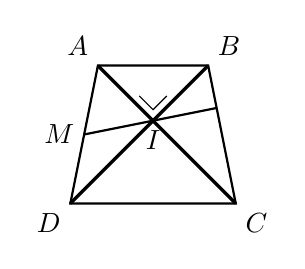
\begin{tikzpicture}[scale=0.35]
			          %projection ($(X)!(B')!(B)$)
			          %nommer chemin 'name path
			          %intersections \path [name intersections={of=d and gb,name=G}];
			          %intersection \path [name intersections={of=d and gb,by=G}];
			          %animation  \draw[visible on=<1>] 
				  %           \draw[visible on=<{2,4}>]
				  %angle arc[radius = 6mm, start angle= 180, end angle= 225] node [below left,pos=0.3]{$\alpha$}
				  %angle \pic [draw,"$\alpha$", angle eccentricity=1.5] {angle = A'--A--B};
				  %perpendiculaire ($(A')!3cm!-90:(A)$)
				  %cercle par point \node [draw] at (A) [circle through=(B)] {};
                                    \coordinate[label=above left:$A$](A) at (-2,2);
                                    \coordinate[label=above right:$B$](B)at (2,2);
                                    \coordinate[label=below right:$C$](C)at (3,-3);
                                    \coordinate[label=below left:$D$](D)at (-3,-3);
                                    \coordinate[label=below:$I$](I)at (0,0);
                                    \coordinate[label=left:$M$](M) at (-2.5,-0.5);
                                    \draw [thick] (A) -- (B) -- (C) -- (D) -- cycle;
                                    \draw [very thick] (A) -- (C) (B) -- (D);
                                    \draw (-0.5,0.9) -- (0,0.4) -- (0.5,0.9);
                                    \draw [thick] (M) -- (I);
                                    \draw [thick] (I) -- (2.3,0.46);
                                    
				  \end{tikzpicture}
				  \end{figure}
			
				  \begin{tcolorbox}[basic] 
				      
				    \smallskip
                                    
				    \hypotheses
					\smallskip		      
				    \these
				    \end{tcolorbox}
		
		
		\column{.53\textwidth}\centering
		
		\underline{Résolution}\\ \flushleft
		
		$\dfrac{|AI|}{|AC|}=\dfrac{|BI|}{|BD|}\quad$ par Thalès (\textcolor{blue}{1.}). \\[1em]
                Or $|AC|=|BD|$ (\textcolor{blue}{2.}), \\[1em]
                $\rightarrow |AI|=|BI|$. \hfill $\qed(a)$ \\[1em]
                Par Pythagore dans les 4 $\Delta$ rectangles,
                
                \begin{align*}
                  &|AD|^2 + |DC|^2 + |CB|^2+|AB|^2, \\[0.5em]
                  &= |AD|^2 + |DI|^2 + |CI|^2 + |BI|^2 + |CI|^2\\&\hspace{20mm} + |AI|^2 + |BI|^2,\\[0.5em]
                  &\begin{cases} |AI|=|BI|, \quad (\textcolor{blue}{a.})\\ |DI|=|CI|.\quad (\textcolor{blue}{a.,\ 2.})\end{cases} \\[0.5em]
                  &= |AD|^2 +  3|AI|^2 + 3|DI|^2 =4|AD|^2.  \hspace{1mm} \qed(b)
                  \end{align*}

                  \bigskip
                  
                 
		%\centering\noindent\rule{2cm}{0.4pt}
                \end{columns}
                     \notedir{%
	   .1 Prouver la thèse.
	   .2 Élément de théorie.
	   .3 Thalès, Pythagore et notions sur produit scalaire..
	   .2 Résolution.
	   .3 Utiliser Thalès sur $\Delta ABI, \Delta DIC$ car.
           .4 $AB\parallel DC$..
           .4 Comme $|AC|=|BD|$ (hypothèse), thèse a) vérifiée..
           .3 Appliquer Pythagore dans $\Delta ABI, \Delta BIC, \Delta DIC, \Delta DIC$..
           .3 $\vect{IM}\cdot\vect{BC}=0 \rightarrow IM\bot BC$..
           .3 Décomposer $\vect{IM}$ et $\vect{BC}$ avec $I$ pour utiliser angle droit..
	   }
         }

    \frame{ 
	  % résolution ex1
	  \begin{columns}[t]
		\column{.54\textwidth}\centering 
		

			\underline{Dessin}\\
			
				  \begin{figure}[h]
				  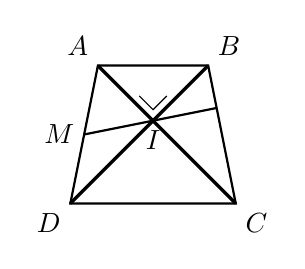
\begin{tikzpicture}[scale=0.35]
			          %projection ($(X)!(B')!(B)$)
			          %nommer chemin 'name path
			          %intersections \path [name intersections={of=d and gb,name=G}];
			          %intersection \path [name intersections={of=d and gb,by=G}];
			          %animation  \draw[visible on=<1>] 
				  %           \draw[visible on=<{2,4}>]
				  %angle arc[radius = 6mm, start angle= 180, end angle= 225] node [below left,pos=0.3]{$\alpha$}
				  %angle \pic [draw,"$\alpha$", angle eccentricity=1.5] {angle = A'--A--B};
				  %perpendiculaire ($(A')!3cm!-90:(A)$)
				  %cercle par point \node [draw] at (A) [circle through=(B)] {};
                                    \coordinate[label=above left:$A$](A) at (-2,2);
                                    \coordinate[label=above right:$B$](B)at (2,2);
                                    \coordinate[label=below right:$C$](C)at (3,-3);
                                    \coordinate[label=below left:$D$](D)at (-3,-3);
                                    \coordinate[label=below:$I$](I)at (0,0);
                                    \coordinate[label=left:$M$](M) at (-2.5,-0.5);
                                    \draw [thick] (A) -- (B) -- (C) -- (D) -- cycle;
                                    \draw [very thick] (A) -- (C) (B) -- (D);
                                    \draw (-0.5,0.9) -- (0,0.4) -- (0.5,0.9);
                                    \draw [thick] (M) -- (I);
                                    \draw [thick] (I) -- (2.3,0.46);
                                    
				  \end{tikzpicture}
				  \end{figure}
			
				  \begin{tcolorbox}[basic] 
				      
				    \smallskip
                                    
				    \hypotheses
					\smallskip		      
				    \these
				    \end{tcolorbox}
		
		
		\column{.53\textwidth}\centering
		
		\underline{Résolution} \flushleft
                 $\vect{IM}=\dfrac{1}{2}\vect{IA}+\dfrac{1}{2}\vect{ID}.$ ($M$ milieu de $[AD]$)\\[0.5em]
                  $\vect{BC}=\vect{BI} + \vect{IC}.$\\
		
                  \begin{align*}
                   & \vect{IM}\cdot\vect{BC}\\[0.5em] &\  = (\dfrac{1}{2}\vect{IA}+\dfrac{1}{2}\vect{ID})\cdot(\vect{BI} + \vect{IC}),\\[0.5em]
                                            &\ =\dfrac{1}{2}(\vect{IA}\cdot\vect{BI} + \vect{IA}\cdot\vect{IC} \\&\hspace{10mm}+ \vect{ID}\cdot\vect{BI} + \vect{ID}\cdot\vect{IC}),\\[0.5em]
                   &\ =\dfrac{1}{2}(|\vect{IA}||\vect{BI}|\cos(90^\circ) + |\vect{IA}||\vect{IC}|\cos(180^\circ) \\&\hspace{7mm}+ |\vect{ID}||\vect{BI}|\cos(0^\circ) + |\vect{ID}||\vect{IC}|\cos(90^\circ)),\\[0.5em]
                   &\ = \dfrac{1}{2}(-|\vect{IA}||\vect{IC}|+ |\vect{ID}||\vect{BI}|),
                    \end{align*}
		
		%\centering\noindent\rule{2cm}{0.4pt}
                  \end{columns}
                          \notedir{%
	   .1 Prouver la thèse.
	   .2 Élément de théorie.
	   .3 Thalès, Pythagore et notions sur produit scalaire..
	   .2 Résolution.
	   .3 Utiliser Thalès sur $\Delta ABI, \Delta DIC$ car.
           .4 $AB\parallel DC$..
           .4 Comme $|AC|=|BD|$ (hypothèse), thèse a) vérifiée..
           .3 Appliquer Pythagore dans $\Delta ABI, \Delta BIC, \Delta DIC, \Delta DIC$..
           .3 $\vect{IM}\cdot\vect{BC}=0 \rightarrow IM\bot BC$..
           .4 Décomposer $\vect{IM}$ et $\vect{BC}$ avec $I$ pour utiliser angle droit..
           .4 Produit scalaire distributif..
           .4 Produit scalaire en termes de longueurs et angles..
         }
       }

       
    \frame{ 
	  % résolution ex1
	  \begin{columns}[t]
		\column{.54\textwidth}\centering 
		

			\underline{Dessin}\\
			
				  \begin{figure}[h]
				  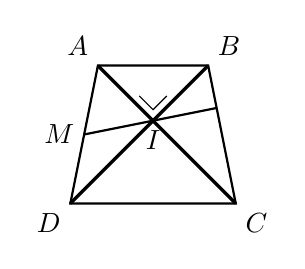
\begin{tikzpicture}[scale=0.35]
			          %projection ($(X)!(B')!(B)$)
			          %nommer chemin 'name path
			          %intersections \path [name intersections={of=d and gb,name=G}];
			          %intersection \path [name intersections={of=d and gb,by=G}];
			          %animation  \draw[visible on=<1>] 
				  %           \draw[visible on=<{2,4}>]
				  %angle arc[radius = 6mm, start angle= 180, end angle= 225] node [below left,pos=0.3]{$\alpha$}
				  %angle \pic [draw,"$\alpha$", angle eccentricity=1.5] {angle = A'--A--B};
				  %perpendiculaire ($(A')!3cm!-90:(A)$)
				  %cercle par point \node [draw] at (A) [circle through=(B)] {};
                                    \coordinate[label=above left:$A$](A) at (-2,2);
                                    \coordinate[label=above right:$B$](B)at (2,2);
                                    \coordinate[label=below right:$C$](C)at (3,-3);
                                    \coordinate[label=below left:$D$](D)at (-3,-3);
                                    \coordinate[label=below:$I$](I)at (0,0);
                                    \coordinate[label=left:$M$](M) at (-2.5,-0.5);
                                    \draw [thick] (A) -- (B) -- (C) -- (D) -- cycle;
                                    \draw [very thick] (A) -- (C) (B) -- (D);
                                    \draw (-0.5,0.9) -- (0,0.4) -- (0.5,0.9);
                                    \draw [thick] (M) -- (I);
                                    \draw [thick] (I) -- (2.3,0.46);
                                    
				  \end{tikzpicture}
				  \end{figure}
			
				  \begin{tcolorbox}[basic] 
				      
				    \smallskip
                                    
				    \hypotheses
					\smallskip		      
				    \these
				    \end{tcolorbox}
		
		
		\column{.53\textwidth}\centering
		
		\underline{Résolution} \flushleft
		
                  \begin{align*}
                   &\ = \dfrac{1}{2}(-|\vect{IA}||\vect{IC}|+ |\vect{IC}||\vect{IA}|),\quad \textcolor{blue}{(2., a.)}\\[0.5em]
                     &\ = 0.\quad \rightarrow IM\bot BC \hspace{20mm} \qed(c)
                    \end{align*}
		
		%\centering\noindent\rule{2cm}{0.4pt}
                  \end{columns}
                          \notedir{%
	   .1 Prouver la thèse.
	   .2 Élément de théorie.
	   .3 Thalès, Pythagore et notions sur produit scalaire..
	   .2 Résolution.
	   .3 Utiliser Thalès sur $\Delta ABI, \Delta DIC$ car.
           .4 $AB\parallel DC$..
           .4 Comme $|AC|=|BD|$ (hypothèse), thèse a) vérifiée..
           .3 Appliquer Pythagore dans $\Delta ABI, \Delta BIC, \Delta DIC, \Delta DIC$..
           .3 $\vect{IM}\cdot\vect{BC}=0 \rightarrow IM\bot BC$..
           .4 Décomposer $\vect{IM}$ et $\vect{BC}$ avec $I$ pour utiliser angle droit..
           .4 Produit scalaire distributif..
           .4 Produit scalaire en termes de longueurs et angles..
           .4 $|\vect{ID}| = |\vect{IC}|$ et  $|\vect{IA}| = |\vect{BI}|$ vu thèse a)..
	   .4 $\vect{IM}\cdot\vect{BC}=0 \rightarrow IM\bot BC$..
         }
         }
	  
             \frame{ 
	  \enonce

	  \vfill\center
	  \underline{Résumé}\\ \flushleft
          \begin{itemize}
	  \item Montrer une égalité de longueur lorsqu'il y a des côtés $\parallel$ $\rightarrow$ Thalès ?
          \item Une somme de carrés de longeur $\rightarrow$ Pythagore ?
            \item Si $\vect{AB}\cdot\vect{CD}=0$ alors $AB\bot CD,$
            \item Si $M$ est milieu du $[AB]$, $\vect{OM}=\frac{1}{2}\vect{OA} + \frac{1}{2}\vect{OB}$,
              \item   $\vect{AB}\cdot\vect{AC}=|\vect{AB}||\vect{AC}|\cos(\widehat{BAC})$.
          \end{itemize}
    }
  
\end{document}

%%% Local Variables:
%%% mode: latex
%%% TeX-master: t
%%% End:
